% Options for packages loaded elsewhere
\PassOptionsToPackage{unicode}{hyperref}
\PassOptionsToPackage{hyphens}{url}
\documentclass[
]{article}
\usepackage{xcolor}
\usepackage[margin=1in]{geometry}
\usepackage{amsmath,amssymb}
\setcounter{secnumdepth}{-\maxdimen} % remove section numbering
\usepackage{iftex}
\ifPDFTeX
  \usepackage[T1]{fontenc}
  \usepackage[utf8]{inputenc}
  \usepackage{textcomp} % provide euro and other symbols
\else % if luatex or xetex
  \usepackage{unicode-math} % this also loads fontspec
  \defaultfontfeatures{Scale=MatchLowercase}
  \defaultfontfeatures[\rmfamily]{Ligatures=TeX,Scale=1}
\fi
\usepackage{lmodern}
\ifPDFTeX\else
  % xetex/luatex font selection
  \setmainfont[]{Cambria}
  \setmonofont[]{Consolas}
\fi
% Use upquote if available, for straight quotes in verbatim environments
\IfFileExists{upquote.sty}{\usepackage{upquote}}{}
\IfFileExists{microtype.sty}{% use microtype if available
  \usepackage[]{microtype}
  \UseMicrotypeSet[protrusion]{basicmath} % disable protrusion for tt fonts
}{}
\makeatletter
\@ifundefined{KOMAClassName}{% if non-KOMA class
  \IfFileExists{parskip.sty}{%
    \usepackage{parskip}
  }{% else
    \setlength{\parindent}{0pt}
    \setlength{\parskip}{6pt plus 2pt minus 1pt}}
}{% if KOMA class
  \KOMAoptions{parskip=half}}
\makeatother
\usepackage{longtable,booktabs,array}
\newcounter{none} % for unnumbered tables
\usepackage{calc} % for calculating minipage widths
% Correct order of tables after \paragraph or \subparagraph
\usepackage{etoolbox}
\makeatletter
\patchcmd\longtable{\par}{\if@noskipsec\mbox{}\fi\par}{}{}
\makeatother
% Allow footnotes in longtable head/foot
\IfFileExists{footnotehyper.sty}{\usepackage{footnotehyper}}{\usepackage{footnote}}
\makesavenoteenv{longtable}
\usepackage{graphicx}
\makeatletter
\newsavebox\pandoc@box
\newcommand*\pandocbounded[1]{% scales image to fit in text height/width
  \sbox\pandoc@box{#1}%
  \Gscale@div\@tempa{\textheight}{\dimexpr\ht\pandoc@box+\dp\pandoc@box\relax}%
  \Gscale@div\@tempb{\linewidth}{\wd\pandoc@box}%
  \ifdim\@tempb\p@<\@tempa\p@\let\@tempa\@tempb\fi% select the smaller of both
  \ifdim\@tempa\p@<\p@\scalebox{\@tempa}{\usebox\pandoc@box}%
  \else\usebox{\pandoc@box}%
  \fi%
}
% Set default figure placement to htbp
\def\fps@figure{htbp}
\makeatother
\setlength{\emergencystretch}{3em} % prevent overfull lines
\providecommand{\tightlist}{%
  \setlength{\itemsep}{0pt}\setlength{\parskip}{0pt}}
\usepackage{bookmark}
\IfFileExists{xurl.sty}{\usepackage{xurl}}{} % add URL line breaks if available
\urlstyle{same}
\hypersetup{
  pdftitle={Telegraph English: Semantic Prompt Compression via Structured Symbolic Rewriting},
  pdfauthor={Mikhail L. Arbuzov; Alexey A. Shvets; Sisong Bei},
  hidelinks,
  pdfcreator={LaTeX via pandoc}}

\title{Telegraph English: Semantic Prompt Compression via Structured
Symbolic Rewriting}
\author{Mikhail L. Arbuzov \and Alexey A. Shvets \and Sisong Bei}
\date{}

\begin{document}
\maketitle

\textbf{Abstract}

We introduce Telegraph English (TE), a compression protocol that
rewrites natural-language text into a symbol-rich, formally-structured
format. Where token-deletion methods like LLMLingua-2 train a classifier
to remove low-information tokens at a fixed ratio, TE performs a full
semantic rewrite: decomposing text into atomic fact lines, substituting
verbose phrases with \textasciitilde40 logical and relational symbols,
and letting the compression ratio adapt to each document's information
density.

A consequence of this design---one we did not initially set out to
achieve---is that compression and semantic chunking collapse into a
single operation. Each output line is an independently addressable fact,
which means the compressed representation is simultaneously a semantic
index. Individual lines can be retained at full fidelity, reduced to
headings, updated with new information, or pruned when they become
redundant. The expensive LLM rewrite happens once; everything after that
is string manipulation.

We evaluate TE on 4,081 question-answer pairs from LongBench-v2 across
five OpenAI models and two difficulty levels. At roughly 50\% token
reduction, TE preserves 99.1\% accuracy on key facts with GPT-4.1 and
outperforms LLMLingua-2 at matched compression ratios on every model and
task tested. The gap widens on smaller models---up to 11 percentage
points on fine-detail tasks---suggesting that explicit relational
structure compensates for limited model capacity. We release the grammar
specification (CC-BY-SA 4.0), compression prompt, benchmark data, and a
reference implementation (MIT License).

\begin{center}\rule{0.5\linewidth}{0.5pt}\end{center}

\subsection{1. Introduction}\label{introduction}

Large language models are increasingly embedded in retrieval-augmented
generation (RAG), multi-agent orchestration, and long-context reasoning
pipelines. In all of these, input cost scales linearly with token count.
Prompt compression---feeding fewer tokens to the model while preserving
the information it needs---has become a practical lever for controlling
latency and cost.

Two families of approach exist. \emph{Extractive} methods select a
subset of tokens or sentences from the input (Jiang et al., 2023; Pan et
al., 2024). \emph{Abstractive} methods paraphrase or summarise it
(Chevalier et al., 2023). LLMLingua-2 (Pan et al., 2024), currently the
strongest published baseline, trains a GPT-4-distilled XLM-RoBERTa-large
classifier to perform binary token classification, deleting tokens below
an importance threshold at a user-specified ratio.

Token deletion works. But it has structural limits that become visible
once you look past the compression ratio.

First, the ratio is fixed regardless of what it's compressing: a dense
technical paragraph gets the same treatment as a verbose preamble.
Second, deleting tokens can sever co-reference chains and destroy
logical connectives, leaving the downstream model to hallucinate the
relationships between surviving fragments. Third, token-deletion methods
are input-only preprocessors---they compress the initial prompt, but
generated output passes uncompressed to the next pipeline stage, so
multi-step agent systems cannot compound the savings. Fourth---and this
is the limitation we find most consequential---token deletion produces
no structure. The output is a degraded copy of the input. It cannot be
indexed, selectively pruned, or dynamically updated. Compressed text is
dead text.

We propose Telegraph English (TE), a different kind of compression.
Rather than selecting which tokens to keep, TE rewrites the passage into
a compact, formally-structured dialect. Before naming the mechanism,
consider what the rewrite looks like. The original sentence

\begin{quote}
\emph{``According to research by Johnson and colleagues (2023), the
application of machine learning techniques to medical diagnostics
resulted in a 27.5\% increase in early detection rates while
simultaneously reducing false positives by approximately 12\% compared
to traditional methods.''}
\end{quote}

becomes, under TE:

\begin{verbatim}
ML→MEDICAL-DIAGNOSTICS: EARLY-DETECTION+27.5% ∧ FALSE-POSITIVE-12% [JOHNSON:2023]
\end{verbatim}

Sixty-eight tokens become fourteen. More importantly, the causal
relationship (\texttt{→}), both quantitative claims, and the citation
are each on record as separate, addressable units --- and the phrase
``application of\ldots{} resulted in'' has collapsed into a single
symbol. That is the move: verbose natural-language framing gives up its
tokens to a compact symbolic dialect, and what survives is
fact-structured rather than token-structured.

The design draws on 19th-century telegraphy, where per-word pricing
forced operators to develop clipped, symbol-rich conventions that
preserved meaning under extreme brevity constraints. The metaphor is
apt, but the mechanism is modern: an LLM performs the rewrite using a
430-line grammar specification as its system prompt.

What makes TE architecturally distinctive is a property that emerges
from the grammar's line-structure rule: compression and semantic
chunking are the same operation. Every TE output line contains exactly
one atomic fact---one claim, one relationship, one datum. This is not a
post-processing step; it is a consequence of how the grammar defines a
legal output. The result is a representation that is simultaneously
compressed, retrieval-ready, and amenable to dynamic management. Three
implications follow:

\begin{enumerate}
\def\labelenumi{\arabic{enumi}.}
\item
  \textbf{Retrieval without re-chunking.} Each atomic line can be
  embedded and retrieved independently. Conventional RAG pipelines
  require a separate chunking stage with arbitrary window sizes and
  overlap heuristics. TE produces chunks whose boundaries are semantic,
  not positional.
\item
  \textbf{Hierarchical context control.} TE output is tagged with
  headings, context scopes, and role markers. An agent assembling a
  prompt under a token budget can retain high-relevance facts at full
  fidelity, reduce moderately relevant sections to their heading tags
  alone, or drop irrelevant sections entirely. This graduated policy
  operates on the structure of the output and requires no additional LLM
  calls.
\item
  \textbf{Dynamic state maintenance.} In multi-turn sessions, facts from
  earlier turns may become stale, redundant, or superseded. Because TE
  facts are individually addressable, they can be updated in-place,
  merged, or pruned. The context window reflects the current state of
  the conversation's knowledge rather than accumulating everything until
  a hard truncation boundary forces a discard.
\end{enumerate}

Our contributions:

\begin{enumerate}
\def\labelenumi{\arabic{enumi}.}
\tightlist
\item
  A formal grammar specification for structured prompt compression
  (Section 3), released under CC-BY-SA 4.0.
\item
  A unified compression-and-chunking framework where semantic
  compression, retrieval-ready indexing, and dynamic context management
  emerge from a single rewriting pass (Sections 3.8, 6.5).
\item
  A large-scale empirical comparison against LLMLingua-2 on 4,081
  key-fact and 801 fine-detail QA pairs across five models (Section 5).
\item
  Evidence --- clean, consistent, and largest where it matters most for
  production deployment --- that semantic rewriting beats token deletion
  on smaller models and on detail-intensive tasks (Section 6).
\item
  A reference implementation with CLI tools for compression,
  benchmarking, and error analysis (Section 7).
\end{enumerate}

\begin{center}\rule{0.5\linewidth}{0.5pt}\end{center}

\subsection{2. Related Work}\label{related-work}

\textbf{Prompt compression.} LLMLingua (Jiang et al., 2023) introduced
budget-constrained prompt compression using perplexity-based token
selection. LLMLingua-2 (Pan et al., 2024) improved on this with a
data-distillation approach: GPT-4 labels token importance on the
MeetingBank corpus, and an XLM-RoBERTa-large classifier learns to
predict which tokens to delete. The compressor is domain-agnostic in
principle, though Pan et al.~note that ``effectiveness decreases on
domains with different token importance distributions'' from the
training data. The key architectural constraint is that the output
remains a degraded subset of the input tokens---no new structure is
introduced.

\textbf{Abstractive compression.} Two lines of work fit here.
AutoCompressors (Chevalier et al., 2023) train summary tokens that
substitute for long contexts; RECOMP (Xu et al., 2023) generates
abstractive summaries tailored to retrieval queries. Both are effective
but lossy by design --- they discard information that cannot be
recovered, and neither produces a structured output that supports
selective manipulation.

\textbf{Structured representations for LLMs.} Chain-of-thought prompting
(Wei et al., 2022) and structured prompting (Hao et al., 2023)
demonstrate that imposing structure on LLM inputs improves reasoning. TE
extends this insight to compression: the hypothesis is that explicit
logical and relational operators help downstream models reconstruct the
intended meaning more reliably than degraded natural language.

\textbf{Context management in agent systems.} Long-running agents face
the problem of context window growth. As exchanges accumulate, the
context must be either truncated (losing early information) or
periodically summarised (requiring additional LLM calls and introducing
lossy abstraction). MemGPT (Packer et al., 2023) addresses this with a
virtual memory hierarchy; Reflexion (Shinn et al., 2023) maintains an
explicit buffer of self-reflections. Both operate on natural-language
representations. TE offers a complementary strategy: structured,
fact-level representations that can be selectively updated and pruned
without further LLM calls.

\textbf{Semantic chunking for RAG.} Standard RAG pipelines split
documents using fixed token windows, recursive splitting, or
sentence-boundary heuristics (Lewis et al., 2020; Gao et al., 2023).
Recent work attempts to align chunk boundaries with topical shifts. TE
sidesteps this problem: compression produces atomic fact lines as a
structural by-product, so no separate chunking stage is needed.

\textbf{Controlled natural languages.} TE shares some conceptual ground
with Attempto Controlled English (Fuchs et al., 2008) and similar
formal-reasoning dialects. The difference is purpose: TE is designed for
compression rather than verification, and its consumer is an LLM rather
than a theorem prover.

\begin{center}\rule{0.5\linewidth}{0.5pt}\end{center}

\subsection{3. The Telegraph English
Grammar}\label{the-telegraph-english-grammar}

The grammar (version 5) lives in a 430-line specification document that
doubles as the system prompt for the LLM-based compressor. We summarise
the key design principles here; the full specification is released as
supplementary material.

\subsubsection{3.1 Foundations}\label{foundations}

Four principles govern the grammar, listed in strict priority order:

\begin{enumerate}
\def\labelenumi{\arabic{enumi}.}
\tightlist
\item
  \textbf{Fidelity over brevity.} No information may be dropped unless
  it is fully inferable from the remaining text. This is the inviolable
  constraint; everything else is subordinate.
\item
  \textbf{Atomic line structure.} Each line contains exactly one claim,
  step, event, or question. Lines are delimited by newlines or
  semicolons.
\item
  \textbf{Upper-case default.} TE is written in upper case unless case
  itself carries information (proper names, code, SI unit symbols).
\item
  \textbf{Target compression \textasciitilde5x} when feasible, but
  correctness, auditability, and reversibility take strict priority over
  token reduction.
\end{enumerate}

\subsubsection{3.2 Symbol Vocabulary}\label{symbol-vocabulary}

TE defines a fixed vocabulary of relational and logical operators. The
full set numbers roughly 40; the table below shows the core symbols that
appear in most compressions:

{\def\LTcaptype{none} % do not increment counter
\begin{longtable}[]{@{}cll@{}}
\toprule\noalign{}
Symbol & Meaning & Example \\
\midrule\noalign{}
\endhead
\bottomrule\noalign{}
\endlastfoot
\texttt{=} & Definition / equality & \texttt{VELOCITY=DISTANCE/TIME} \\
\texttt{→} & Causation / flow & \texttt{HEAT→EXPANSION} \\
\texttt{⇒} & Logical implication & \texttt{RAIN⇒WETNESS} \\
\texttt{∴} & Therefore / conclusion &
\texttt{X\textgreater{}Y\ ∧\ Y\textgreater{}Z\ ∴\ X\textgreater{}Z} \\
\texttt{∵} & Because / reason & \texttt{MOTOR-FAILURE\ ∵\ OVERLOAD} \\
\texttt{↑} / \texttt{↓} & Increase / decrease & \texttt{TEMPERATURE↑} \\
\texttt{∧} / \texttt{∨} / \texttt{¬} & AND / OR / NOT & \texttt{A∧B},
\texttt{¬EVIDENCE} \\
\texttt{≈} / \texttt{≠} & Approximate / not equal &
\texttt{COST≈USD10M} \\
\texttt{VS} & Contrast (never causal) & \texttt{MODEL-A\ VS\ MODEL-B} \\
\end{longtable}
}

Each symbol has a single, non-interchangeable meaning. The grammar caps
symbol density at three consecutive symbols per line---a readability
constraint learned from early iterations where dense symbol chains
became opaque even to GPT-4.

\subsubsection{3.3 Tagging System}\label{tagging-system}

Structured tags handle temporal state (\texttt{PAST:}, \texttt{NOW:},
\texttt{FUTURE:}), modality (\texttt{LIKELY:}, \texttt{POSSIBLE:},
\texttt{CONF=0.87}), roles (\texttt{AGENT:}, \texttt{PATIENT:},
\texttt{INSTRUMENT:}), scope (\texttt{CTX:} for shared context), and
structured content types (\texttt{DEF:} for definitions, \texttt{Q:} /
\texttt{A:} for questions and answers). These tags serve double duty:
they compress verbose natural-language framing into single tokens, and
they provide the structural handles that enable downstream selective
retrieval and context management.

\subsubsection{3.4 Domain-Specific
Conventions}\label{domain-specific-conventions}

The grammar standardises formatting for quantities
(\texttt{VAR=VALUEUNIT}, SI case rules), citations
(\texttt{{[}AUTH:YEAR{]}}, \texttt{DOI:}, \texttt{ARXIV:}), financial
data (\texttt{USD10.5\ M}, \texttt{Y/Y+5\%}, \texttt{+2.5PT} for
percentage points), and URLs (\texttt{URL:https://...}).

\subsubsection{3.5 Quality Gate}\label{quality-gate}

Every TE output must pass a 12-point verification checklist covering
formatting consistency, symbol precision, abbreviation policy, number
formatting, information preservation, and citation integrity. The
checklist is embedded directly in the compression prompt, so the
compressor model self-verifies before returning output.

\subsubsection{3.6 Information Distillation
Process}\label{information-distillation-process}

The specification prescribes a six-pass distillation: (1) concept
identification, (2) claim extraction, (3) relation mapping, (4)
redundancy elimination, (5) numerical verification, and (6) citation
cross-checking. This is a prescribed reasoning sequence for the
compressor model, not a multi-call pipeline---all six passes happen
within a single LLM inference.

\subsubsection{3.7 Compression Example}\label{compression-example}

A single sentence, expanded and compressed:

\textbf{Original (68 tokens):} \emph{``According to research by Johnson
and colleagues (2023), the application of machine learning techniques to
medical diagnostics resulted in a 27.5\% increase in early detection
rates while simultaneously reducing false positives by approximately
12\% compared to traditional methods.''}

\textbf{TE (14 tokens):}

\begin{verbatim}
MACHINE-LEARNING→MEDICAL-DIAGNOSTICS: EARLY-DETECTION+27.5% ∧ FALSE-POSITIVE-12% [JOHNSON:2023]
\end{verbatim}

Compression ratio: 4.9x. The causal relationship, both quantitative
claims, and the citation are all preserved. The \texttt{→} operator
makes the causal direction explicit---something the original expressed
with the phrase ``application of\ldots{} resulted in,'' which is six
tokens doing the work of one symbol.

\subsubsection{3.8 Compression as Semantic
Chunking}\label{compression-as-semantic-chunking}

Here is the property we consider most architecturally significant:
compression and semantic chunking are not separate stages. They are the
same operation.

Consider a multi-paragraph clinical trial summary compressed into TE:

\begin{verbatim}
H1: CLINICAL-TRIAL OUTCOMES
CTX: PHASE-III RANDOMISED CONTROLLED-TRIAL(RCT); N=2400
  PRIMARY-ENDPOINT: MORTALITY↓23% VS PLACEBO; p<0.001 [SMITH:2024]
  SECONDARY-ENDPOINT: HOSPITALIZATION↓18%; p=0.003
  ADVERSE-EVENTS: NAUSEA=12% ∧ HEADACHE=8% ∧ SERIOUS=2.1%
H1: SUBGROUP-ANALYSIS
  AGE>65: MORTALITY↓31% (STRONGER-EFFECT)
  AGE<65: MORTALITY↓14% (WEAKER-EFFECT)
  CONF=0.92 FOR INTERACTION-EFFECT
H1: LIMITATIONS
  FOLLOW-UP=18 MONTHS; LONG-TERM-EFFECTS UNKNOWN
  EXCLUSION: PATIENTS WITH RENAL-IMPAIRMENT
\end{verbatim}

Each line is a fact. Each heading is a section boundary. Each
\texttt{CTX:} block defines a scope. This structure---which falls out of
the grammar's line-structure rule, not from any additional
processing---enables three things that token-deleted text cannot
support:

\textbf{Selective retrieval.} A query about adverse events retrieves
exactly the \texttt{ADVERSE-EVENTS} line and its \texttt{CTX:} scope. No
sliding-window heuristic, no overlap parameter, no risk of splitting a
relevant fact across chunk boundaries. The semantic boundaries are
intrinsic to the format.

\textbf{Graduated compression-on-read.} When assembling a prompt under a
tight token budget, an agent can apply different policies to different
sections: keep the lines most relevant to the current query at full
fidelity; retain only the heading tags (\texttt{H1:\ LIMITATIONS}) for
moderately relevant sections, preserving topic structure at near-zero
cost; drop irrelevant sections entirely. This second-stage compression
is semantically principled---it operates on identified sections, not on
token positions.

\textbf{Continuous state refinement.} During a conversation, facts from
earlier turns can be revised without re-compressing the source: -
\textbf{Update}: replace \texttt{PRIMARY-ENDPOINT:\ MORTALITY↓23\%} with
a corrected figure from a follow-up. - \textbf{Merge}: combine two
related facts into a single tighter line when the distinction no longer
matters. - \textbf{Prune}: remove claims about exclusion criteria once
the conversation has moved past trial design. - \textbf{Promote/demote}:
expand a heading-collapsed section when it becomes relevant again, or
collapse a fully expanded section that the session has moved beyond.

The context window reflects the current state of knowledge, not a
chronological log. We formalise this as the \textbf{compress-once,
manage-continuously} principle: the expensive LLM rewriting pass happens
once per document; subsequent manipulation---re-ranking, filtering,
updating, re-assembly---is cheap string operations requiring no further
LLM calls.

\begin{center}\rule{0.5\linewidth}{0.5pt}\end{center}

\subsection{4. Experimental Setup}\label{experimental-setup}

\subsubsection{4.1 Dataset}\label{dataset}

LongBench-v2 (Bai et al., 2024) supplies the source corpus: 503
long-context documents. We filter to three categories suitable for
factual QA---Single-Document QA, Multi-Document QA, and Long-Dialogue
History Understanding---which leaves 339 documents. NLTK sentence
tokenisation chunks each one into segments of at most 1,000 words,
producing 4,081 chunk-level evaluation units.

\subsubsection{4.2 Compression}\label{compression}

Each chunk is compressed into TE using the v5 grammar prompt with
OpenAI's o4-mini model. We measure token counts with tiktoken
(cl100k\_base encoding). The mean compression ratio is 0.585---a 41.5\%
token reduction---with a range spanning 0.13 to 1.57. That upper end
deserves explanation: rare, very short inputs that are already
informationally dense occasionally \emph{expand} under TE, because the
grammar's fidelity-first principle prohibits dropping information even
when doing so would reduce token count. This is a feature, not a
failure. The full distribution is shown in Figures 1 and 2.

\begin{figure}
\centering
\pandocbounded{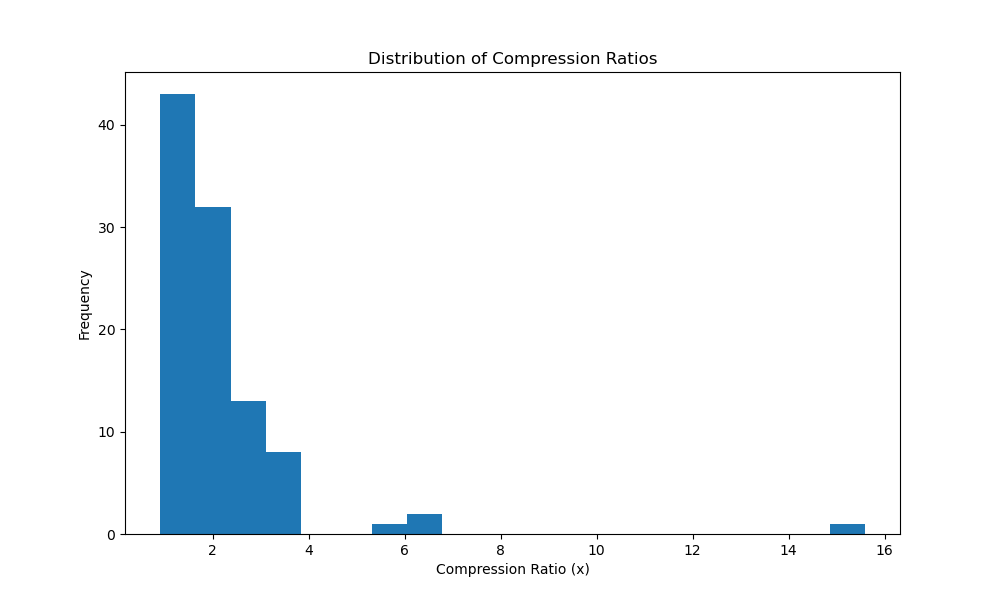
\includegraphics[keepaspectratio,alt={Distribution of compression ratios across 4,081 LongBench-v2 chunks compressed with Telegraph English (o4-mini, tiktoken cl100k\_base). Mean 0.585, range 0.13--1.57. The right tail above 1.0 corresponds to short, dense inputs that expand under TE because the grammar's fidelity-first rule prohibits dropping information even when doing so would reduce token count.}]{figures/figure1_compression_ratio.png}}
\caption{Distribution of compression ratios across 4,081 LongBench-v2
chunks compressed with Telegraph English (o4-mini, tiktoken
cl100k\_base). Mean 0.585, range 0.13--1.57. The right tail above 1.0
corresponds to short, dense inputs that expand under TE because the
grammar's fidelity-first rule prohibits dropping information even when
doing so would reduce token count.}
\end{figure}

\begin{figure}
\centering
\pandocbounded{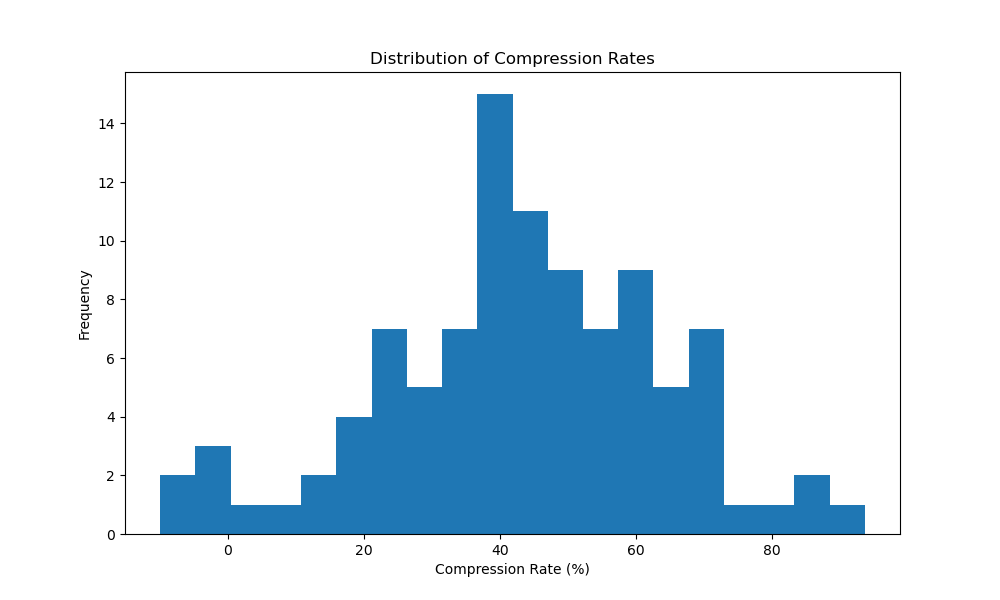
\includegraphics[keepaspectratio,alt={Distribution of per-chunk compression rate (1 - ratio) over the same corpus. The median chunk loses roughly 43\% of its tokens; the bottom decile loses very little, reflecting TE's adaptive behaviour on already-dense inputs.}]{figures/figure2_compression_rate.png}}
\caption{Distribution of per-chunk compression rate (1 - ratio) over the
same corpus. The median chunk loses roughly 43\% of its tokens; the
bottom decile loses very little, reflecting TE's adaptive behaviour on
already-dense inputs.}
\end{figure}

For the LLMLingua-2 baseline, the same chunks are compressed using the
publicly available \texttt{llmlingua} package at two retention rates:
0.50 (50\% of tokens kept) and 0.33 (33\% kept).

\subsubsection{4.3 QA Evaluation Protocol}\label{qa-evaluation-protocol}

We design a multiple-choice protocol that isolates comprehension: can a
model answer a factual question correctly when reading compressed text
instead of the original? Five steps:

\begin{enumerate}
\def\labelenumi{\arabic{enumi}.}
\item
  \textbf{QA generation.} GPT-4.1 generates a factual question-answer
  pair from the original chunk. The answer must be verbatim from the
  passage. A semantically equivalent but lexically distinct ``modified
  answer'' is also produced---this prevents simple string matching from
  inflating scores.
\item
  \textbf{Distractor generation.} GPT-4.1 (temperature 0.7) generates
  three plausible but incorrect answers, matched in style, length, and
  specificity to the correct answer.
\item
  \textbf{Choice shuffling.} The modified answer and three distractors
  are shuffled into a four-option question. The correct answer's
  position is recorded as \texttt{gold\_idx}.
\item
  \textbf{Evaluation on original text.} The evaluation model receives
  the original chunk and selects an answer.
\item
  \textbf{Evaluation on compressed text.} The same model receives the
  compressed chunk---TE or LLMLingua-2---and selects an answer.
\end{enumerate}

Accuracy is the fraction of correct selections. An \emph{error} is a
case where the model answers correctly on the original but incorrectly
on the compressed version---the compression caused the failure.

\subsubsection{4.4 Test Suites}\label{test-suites}

Two suites probe different levels of information preservation:

\textbf{key\_facts} (4,081 QA pairs): Questions target core
concepts---headline findings, main claims, central arguments.
Distractors are generically plausible.

\textbf{fine\_facts} (801 QA pairs): Questions are adversarially
designed to target information that lossy compression is most likely to
destroy: precise numerical qualifiers, conditional statements, boundary
conditions, secondary details. Distractors are near-miss
variants---changing 4.8\% to 4.3\%, for instance---that can only be
distinguished with access to the exact original detail.

\subsubsection{4.5 Models}\label{models}

Five OpenAI models spanning the capability-cost spectrum:

{\def\LTcaptype{none} % do not increment counter
\begin{longtable}[]{@{}ll@{}}
\toprule\noalign{}
Model & Role \\
\midrule\noalign{}
\endhead
\bottomrule\noalign{}
\endlastfoot
GPT-4.1 & QA generation + MC evaluation \\
GPT-4o & MC evaluation \\
GPT-4o-mini & MC evaluation \\
GPT-4.1-nano & MC evaluation \\
Fine-tuned GPT-4o & MC evaluation \\
\end{longtable}
}

Different suites use different model subsets. GPT-4.1, GPT-4o-mini, and
GPT-4.1-nano carry the key\_facts evaluation; GPT-4o and GPT-4o-mini
handle the adversarial fine\_facts suite. The fine-tuned GPT-4o variant
is reported in the cost analysis (§6.4) but is not used as a separate
accuracy benchmark --- it serves as a sanity check that fine-tuning on
the original distribution does not change comparative behaviour at
compression-decoded inputs.

\begin{center}\rule{0.5\linewidth}{0.5pt}\end{center}

\subsection{5. Results}\label{results}

\subsubsection{5.1 Key Facts Accuracy}\label{key-facts-accuracy}

Table 1 reports accuracy on the key\_facts suite.

\textbf{Table 1.} Key facts accuracy (4,081 QA pairs). TE = Telegraph
English (\textasciitilde50\% compression). LLML2-50 = LLMLingua-2 at
50\% retention. Drop measured in percentage points (pp) relative to
original.

{\def\LTcaptype{none} % do not increment counter
\begin{longtable}[]{@{}llllll@{}}
\toprule\noalign{}
Model & Original & TE & LLML2-50 & TE Drop & LLML2-50 Drop \\
\midrule\noalign{}
\endhead
\bottomrule\noalign{}
\endlastfoot
GPT-4.1 & 1.000 & \textbf{0.991} & 0.990 & -0.9 pp & -1.0 pp \\
GPT-4o-mini & 0.991 & \textbf{0.957} & 0.946 & -3.4 pp & -4.5 pp \\
GPT-4.1-nano & 0.980 & \textbf{0.950} & 0.949 & -3.0 pp & -3.1 pp \\
\end{longtable}
}

On headline facts, TE matches or edges out LLMLingua-2 across the board.
The accuracy loss is negligible for GPT-4.1 --- less than a percentage
point while halving the token count. The gap widens on smaller models:
1.1 pp on GPT-4o-mini, with the same direction at GPT-4.1-nano. Not
dramatic. But consistent --- the direction never reverses across
configurations.

\subsubsection{5.2 Fine Facts Accuracy}\label{fine-facts-accuracy}

Table 2 reports accuracy on the adversarial fine\_facts suite.

\textbf{Table 2.} Fine facts accuracy (801 QA pairs). LLML2-33 =
LLMLingua-2 at 33\% retention.

{\def\LTcaptype{none} % do not increment counter
\begin{longtable}[]{@{}llllll@{}}
\toprule\noalign{}
Model & Original & TE & LLML2-50 & TE Drop & LLML2-50 Drop \\
\midrule\noalign{}
\endhead
\bottomrule\noalign{}
\endlastfoot
GPT-4o & 0.996 & \textbf{0.965} & 0.933 & -3.1 pp & -6.3 pp \\
GPT-4o-mini & 0.938 & \textbf{0.843} & 0.820 & -9.5 pp & -11.8 pp \\
\end{longtable}
}

Fine details are harder. Compression loss runs 3-4x higher than on key
facts, regardless of method. But TE holds an advantage: 3.2 pp over
LLMLingua-2 on GPT-4o, 2.3 pp on GPT-4o-mini at matched 50\% retention.
Against the more aggressive LLMLingua-2 at 33\% retention, the story is
starker---TE's lead grows to roughly 11 pp on GPT-4o-mini, where
LLMLingua-2 drops a full 21 pp from baseline. That configuration is
where token deletion starts to break down: it's removing tokens that
carry the very details the questions probe.

\subsubsection{5.3 Accuracy Hierarchy}\label{accuracy-hierarchy}

Across all models and tasks, the ranking holds without exception:

\begin{enumerate}
\def\labelenumi{\arabic{enumi}.}
\tightlist
\item
  \textbf{Original (uncompressed)} --- baseline
\item
  \textbf{Telegraph English (\textasciitilde50\%)} --- 1-3 pp drop on
  key facts; 3-11 pp on fine facts
\item
  \textbf{LLMLingua-2 at 50\%} --- consistently behind TE
\item
  \textbf{LLMLingua-2 at 33\%} --- significant accuracy loss, up to 21
  pp on fine facts with smaller models
\end{enumerate}

\subsubsection{5.4 Compression Statistics}\label{compression-statistics}

TE's mean compression ratio of 0.585 (std = 0.254) hides a wide spread.
Half the corpus sits between 0.41 and 0.74; the median is 0.57.
Documents dense with technical content or data tables resist compression
--- narrative text, by contrast, can yield ratios of 5:1 or better. This
variability is the point. The compression adapts to the information
density rather than imposing a fixed ratio. Fidelity-first design means
the ratio is an outcome, not a parameter.

\subsubsection{5.5 Error Analysis}\label{error-analysis}

We examined the 187 items (4.6\%) where GPT-4.1-nano---the weakest
model---answered correctly on the original but incorrectly on the
TE-compressed version. These error cases have a mean compression ratio
of 0.531, slightly more compressed than the population mean, which
suggests that aggressive compression and error risk are correlated. The
failures cluster around fine details: dates, measurement units,
conditional qualifications, and numerical relationships where the TE
compression either abbreviates a critical modifier or collapses a
distinction that the question specifically probes.

One characteristic failure: a legal document chunk where TE compressed
``no later than 30 calendar days after receipt of written notice'' into
\texttt{DEADLINE=30D-AFTER-NOTICE}. The question asked whether the
deadline was measured in calendar days or business days. The
\texttt{30D} abbreviation is ambiguous on this point---the grammar's
default day notation does not distinguish calendar from business days.
This is a genuine limitation of the symbol vocabulary, not a compressor
error; the grammar lacks the granularity to preserve this distinction in
its current form.

\begin{center}\rule{0.5\linewidth}{0.5pt}\end{center}

\subsection{6. Analysis}\label{analysis}

\subsubsection{6.1 Why Semantic Rewriting Outperforms Token
Deletion}\label{why-semantic-rewriting-outperforms-token-deletion}

Four mechanisms explain the pattern in the results. They are not ranked;
different mechanisms dominate in different regimes.

\textbf{Semantic unit preservation.} Token deletion operates at the
token level --- and that is the problem. It can split multi-word
expressions, sever noun-modifier pairs, strand a number from its unit.
TE works one level up: related concepts are grouped into hyphenated
compounds (\texttt{EARLY-DETECTION-RATE}), and complete claims occupy
single lines. The unit of compression is the claim, not the token.

\textbf{Explicit logical structure.} Delete a connective like
``therefore'' or ``in contrast to'' and the downstream model has to
guess the relationship from what remains. TE refuses to offer the guess:
\texttt{∴} for conclusion, \texttt{VS} for contrast, \texttt{→} for
causation --- each unambiguous, each preserved regardless of what else
is removed. Reviewers familiar with LLMLingua-2's failure modes will
recognise this as the reconstruction-from-fragments problem, and it is
the failure mode TE's symbols most directly address.

\textbf{Co-reference stability.} Because TE is one-claim-per-line, with
every entity in upper-case and referenced by name, pronouns largely
disappear. Token deletion can strand a pronoun whose antecedent has been
removed --- a surprisingly common failure where the compressed text is
grammatical but its referents are unrecoverable. TE's referents, by
construction, do not get stranded.

\textbf{Adaptive compression.} A fixed-ratio method compresses a dense
technical paragraph as aggressively as a repetitive introduction. TE
does not. Dense passages resist compression and emerge at ratios near
1.0; verbose passages compress to 0.2 or below. Whether this
density-sensitive behaviour transfers to non-technical genres is an open
question --- our corpus leans technical --- but within that corpus, the
method spends its budget where the information lives.

The four mechanisms are not independent. Semantic-unit preservation
makes co-reference stability easier to achieve. Explicit logical
structure depends on having claim-level units to operate on. Adaptive
compression is a consequence of fidelity-first design rather than a
separate property. The result is that LLMLingua-2 cannot match TE by
adopting any single one of these --- the architectural commitments
interlock.

\subsubsection{6.2 The Small-Model Effect}\label{the-small-model-effect}

The TE advantage grows as model capacity shrinks. GPT-4.1 barely notices
the difference between TE and LLMLingua-2 on key facts; GPT-4.1-nano and
GPT-4o-mini show a wider gap, and on fine facts the divergence becomes
substantial.

The likely explanation is capacity-dependent. Smaller models have less
ability to reconstruct implicit relationships from token-deleted
fragments. TE compensates by offloading the reconstruction work to the
compression stage --- the evaluation model receives a representation
where the relationships are already marked, rather than having to
hallucinate them from sparse clues. This has practical weight: smaller
models are precisely the ones deployed in cost-sensitive production
pipelines, which is where prompt compression earns its keep.

\subsubsection{6.3 The Fine-Facts Gap}\label{the-fine-facts-gap}

Key facts survive both compression methods reasonably well. Central
claims and prominent findings carry high information density and are
often redundantly signalled; even aggressive token deletion tends to
preserve them. Fine details are stubborn in a different way. Precise
numerical qualifiers, conditional caveats, secondary attributions ---
these are exactly the tokens that an entropy-based classifier flags as
low-importance when considered in isolation. A number like ``4.8\%'' may
look dispensable next to the surrounding prose. But if the question asks
whether the figure was 4.8\% or 4.3\%, that token is the entire answer.

TE's claim-level decomposition and explicit numerical formatting
(\texttt{+27.5\%}, \texttt{CONF=0.87}, \texttt{Y/Y+12.3\%}) are designed
to preserve these details. The grammar treats every number as a
first-class citizen: numbers are never abbreviated, always attached to
their units, and always placed in a structured format that a downstream
model can parse unambiguously.

\subsubsection{6.4 Pipeline-Level Cost}\label{pipeline-level-cost}

There is a structural difference between the two methods that the
accuracy comparison alone obscures: LLMLingua-2 operates as an
input-only preprocessor. It compresses the initial prompt; generated
output passes uncompressed to subsequent stages. TE can persist as a
native format throughout a pipeline.

Consider a five-step agent pipeline with 2,000 tokens of initial context
and five generation steps averaging 400 tokens each. At \$10 per million
tokens:

{\def\LTcaptype{none} % do not increment counter
\begin{longtable}[]{@{}llll@{}}
\toprule\noalign{}
Method & Total tokens & Cost / 1K calls & Savings \\
\midrule\noalign{}
\endhead
\bottomrule\noalign{}
\endlastfoot
Original & 4,000 & \$40 & --- \\
LLMLingua-2 & \textasciitilde3,300 & \$33 & \$7 \\
Telegraph English & \textasciitilde1,600 & \$16 & \$24 \\
\end{longtable}
}

The savings compound because each stage operates on TE-formatted text.
LLMLingua-2 compresses only the first stage's input; the remaining four
stages process uncompressed output at full token cost.

\subsubsection{6.5 Beyond Static Compression: Semantic Chunking and
Dynamic
Context}\label{beyond-static-compression-semantic-chunking-and-dynamic-context}

The results in Sections 5.1--5.4 measure TE as a static compression
method---compress once, read once, evaluate. This is the fair comparison
against LLMLingua-2, and it's where the benchmark numbers live. But we
think the more consequential property of TE is not its compression
ratio; it's the \emph{structure} of its output.

\textbf{Unifying compression and chunking.} Conventional RAG systems run
documents through two stages: chunking (splitting into fixed-size
segments for embedding) and optional compression (reducing each chunk's
token count). These stages have different objectives and can
interfere---a chunk boundary splits a sentence, and compression then
deletes the tokens needed to reconstruct it. TE collapses both stages
into one. Each output line is a complete semantic unit; the chunking
boundaries \emph{are} the compression output. A TE-compressed document
is immediately embeddable at the line level, no post-processing
required.

The practical consequence for retrieval precision is straightforward.
Fixed-window chunking (say, 512 tokens with overlap) inevitably includes
irrelevant context within each chunk and risks splitting relevant
information across boundaries. TE surfaces exactly the facts a query
matches, at the granularity of individual claims.

\textbf{Hierarchical context budgeting.} Because the output is tagged
with headings (\texttt{H1:}, \texttt{H2:}), context scopes
(\texttt{CTX:}), and role markers, a context-assembly system can make
graduated decisions about inclusion. For a given token budget:

\begin{itemize}
\tightlist
\item
  \emph{Full fidelity}: all atomic lines for the most relevant sections.
\item
  \emph{Heading-only}: just the \texttt{H1:} / \texttt{H2:} tags for
  moderately relevant sections---topic structure preserved at near-zero
  token cost.
\item
  \emph{Omission}: irrelevant sections dropped entirely.
\end{itemize}

This graduated policy can achieve very high total compression (10-50x)
when only a fraction of the document is relevant, while maintaining full
detail where it matters. The policy operates on the TE output's
structure. No LLM call needed.

\textbf{Dynamic state in agentic sessions.} This is, we believe, the
application with the most unrealised potential. Long-running agent
sessions accumulate context over many exchanges. The standard solutions
are blunt instruments: hard truncation drops the oldest tokens
regardless of relevance; periodic summarisation requires an LLM call and
is irreversible.

TE enables something finer. Because context is already decomposed into
tagged atomic facts, an agent can maintain a living context state:

\begin{itemize}
\tightlist
\item
  \textbf{Fact updates}: new information replaces the old line in-place,
  not appended alongside it.
\item
  \textbf{Redundancy pruning}: a fact that has been acted upon and is no
  longer needed gets removed---the information it carried is captured in
  subsequent facts.
\item
  \textbf{Scope closure}: when a topic is resolved, its entire
  \texttt{CTX:} block collapses to a heading. The \emph{that} is
  preserved; the \emph{what} and \emph{why} are released.
\item
  \textbf{Priority re-ranking}: facts reorder by current relevance,
  placing the most important context at the top of the prompt where
  transformer attention is strongest.
\end{itemize}

Context growth is controlled not by discarding the oldest tokens, but by
continuously refining the set of active facts. This is cheap---string
manipulation, no LLM calls---and semantically principled, operating on
identified facts rather than arbitrary token boundaries.

We call this the \textbf{compress-once, manage-continuously} principle.
The cost profile is asymmetric by design: one expensive LLM rewrite per
document, then indefinite cheap manipulation of the structured output.

\begin{center}\rule{0.5\linewidth}{0.5pt}\end{center}

\subsection{7. Implementation}\label{implementation}

The reference implementation is a Python package with five pipeline
stages:

\begin{enumerate}
\def\labelenumi{\arabic{enumi}.}
\tightlist
\item
  \textbf{Compression} (\texttt{telegrapher.compression}): synchronous
  (Chat API) and asynchronous (Batch API) compression of LongBench-v2
  documents using the TE grammar prompt.
\item
  \textbf{Review} (\texttt{telegrapher.review}): automated quality
  review via Claude, producing structured JSON scores (0-10) with
  identified strengths, weaknesses, and original/compressed example
  pairs.
\item
  \textbf{QA Benchmarking} (\texttt{telegrapher.benchmark}): end-to-end
  QA generation, distractor creation, multiple-choice evaluation, and
  accuracy computation.
\item
  \textbf{Baseline Evaluation}
  (\texttt{telegrapher.benchmark.llml2\_eval}): evaluation of
  LLMLingua-2-compressed text against the same QA pairs.
\item
  \textbf{Error Analysis}
  (\texttt{telegrapher.benchmark.error\_analysis}): identification and
  reporting of compression-induced failures, with detailed case-level
  output.
\end{enumerate}

Each stage is accessible as both a CLI command
(\texttt{python\ -m\ cli.compress}, \texttt{python\ -m\ cli.bench},
\ldots) and an importable library function; configuration is centralised
in a single module. The grammar specification is released under CC-BY-SA
4.0, the implementation under the MIT License, and the benchmark data
under CC0.

\begin{center}\rule{0.5\linewidth}{0.5pt}\end{center}

\subsection{8. Limitations}\label{limitations}

\textbf{LLM-dependent compression.} TE requires an LLM call per chunk,
adding latency and cost at compression time. This cost is amortised when
compressed text is reused across multiple retrievals or pipeline
invocations, but it makes TE poorly suited for compressing ephemeral
inputs that will be read once and discarded.

\textbf{Proprietary evaluation models.} Our benchmark relies on OpenAI
models that are not open-weight. This limits reproducibility; future
work should extend the evaluation to open models (Llama, Mistral,
Gemma).

\textbf{English only.} The grammar and all benchmarks are
English-language. Adapting the symbol vocabulary and abbreviation
conventions to other languages---particularly agglutinative or
logographic ones---is non-trivial.

\textbf{Compressor model sensitivity.} The quality of TE output depends
on the model performing the rewrite. We use o4-mini for cost efficiency.
A more capable compressor would likely produce better results; a weaker
one would introduce errors. We have not yet mapped this sensitivity
curve.

\textbf{QA generation bias.} Both the QA pairs and the evaluation are
produced by OpenAI models, creating a risk of systematic bias. An ideal
evaluation would include human-written questions or a diverse set of QA
generators.

\textbf{Dynamic context management is not yet benchmarked.} The semantic
chunking and dynamic state management capabilities described in Sections
3.8 and 6.5 are architectural arguments supported by the structure of
the TE output, not empirical results from a multi-turn evaluation. We
have demonstrated that the format supports these operations; we have not
yet measured their effect on accuracy or efficiency over extended
sessions. This is the most important gap in the current evaluation and
the most pressing direction for future work.

\textbf{Comparison scope.} We benchmark against LLMLingua-2 only ---
currently the strongest published baseline at the compression ratios we
operate in. A broader comparison against AutoCompressors, RECOMP, and
more recent methods would strengthen the claims.

\begin{center}\rule{0.5\linewidth}{0.5pt}\end{center}

\subsection{9. Future Work}\label{future-work}

The compress-once, manage-continuously principle is currently a design
argument. Validating it --- and the related architectural claims of §6.5
--- requires benchmarks that don't yet exist. The list below sketches
the priority directions, in roughly the order we expect to pursue them.

\textbf{Multi-turn context management benchmarks.} Sessions of 50--500
exchanges, with TE's fact-level update/prune strategy compared against
truncation, periodic summarisation, and hybrid approaches. Key metrics:
accuracy on questions about earlier turns, token efficiency over session
length, latency of context operations.

\textbf{Retrieval evaluation.} TE's claim that atomic-line structure
improves RAG retrieval precision needs validation against standard
retrieval benchmarks, measuring recall@k and downstream answer accuracy
for line-level vs.~window-level chunking.

\textbf{Key token preservation theory.} A formal analysis of which
semantic units contribute most to downstream accuracy, which would
inform adaptive compression thresholds and provide a principled basis
for the hierarchical budgeting policy.

\textbf{Domain-specific grammars.} Specialised TE dialects for legal,
biomedical, and financial domains where precision requirements
differ---and where the hierarchical context management is arguably most
valuable (e.g., maintaining a living case-law context across a multi-day
legal research session).

\textbf{Embedding geometry.} How does TE compression affect vector
embedding structure in RAG pipelines? Do compressed and uncompressed
vectors remain meaningfully similar? Do line-level TE embeddings produce
better retrieval than paragraph-level embeddings of uncompressed text?

\textbf{Multilingual extension.} Adapting the grammar to languages with
different morphological structures.

\textbf{TE-to-TE summarisation.} Iterative compression where
already-compressed TE text is further condensed at the section or
heading level, automating the graduated compression-on-read strategy.

\textbf{Confidence-based adaptive compression.} Using the \texttt{CONF=}
tag to dynamically adjust compression aggressiveness based on the
compressor model's uncertainty, and to inform which facts are safe to
prune during context management.

\begin{center}\rule{0.5\linewidth}{0.5pt}\end{center}

\subsection{10. Conclusion}\label{conclusion}

Telegraph English demonstrates that structured semantic rewriting is a
viable alternative to token deletion for prompt compression --- and, on
the evidence presented here, a better one. A formal grammar with
explicit logical operators, atomic line structure, and document-adaptive
compression preserves factual accuracy more reliably than LLMLingua-2
across every model and task difficulty we tested. The advantage is
largest where compression matters most practically: on smaller, cheaper
models and on fine-grained details.

The quantitative comparison may not be the most interesting part of this
paper. Token-deletion methods treat compression as a one-time lossy
reduction; the output is smaller, but still unstructured --- a degraded
copy of the input with no internal organisation. TE produces something
different: a representation where every line is an identified fact,
every section is tagged, and every relationship is marked with an
explicit symbol. This structure makes the output not just smaller but
more \emph{useful} --- more retrievable, more auditable, more
maintainable over time.

The compress-once, manage-continuously principle is, at this stage, an
architectural argument rather than an empirical result. We have shown
that the format supports selective retention, hierarchical compression,
fact-level updates, and scope-based pruning. We have not yet measured
the downstream effects of these operations in production agent systems.
That measurement is the obvious next step, and it is the one most likely
to determine whether TE becomes a practical tool for long-running
context management or remains a compression method with an interesting
side property.

What we can say now: a 40-symbol vocabulary, a one-claim-per-line
discipline, and a fidelity-first design principle together achieve
compression competitive with statistical methods while producing output
that a downstream system can actually work with. Whether ``work with''
scales to the dynamic context scenarios we've described is the open
question this paper is designed to provoke.

\begin{center}\rule{0.5\linewidth}{0.5pt}\end{center}

\subsection{References}\label{references}

Bai, Y., et al.~(2024). LongBench v2: Towards Deeper Understanding and
Reasoning on Realistic Long-context Multitasks. \emph{arXiv preprint
arXiv:2412.15204}.

Chevalier, A., Wettig, A., Ajith, A., \& Chen, D. (2023). Adapting
Language Models to Compress Contexts. \emph{Proceedings of EMNLP 2023}.

Fuchs, N. E., Kaljurand, K., \& Kuhn, T. (2008). Attempto Controlled
English for Knowledge Representation. \emph{Reasoning Web}, LNCS 5224,
104--124.

Gao, Y., et al.~(2023). Retrieval-Augmented Generation for Large
Language Models: A Survey. \emph{arXiv preprint arXiv:2312.10997}.

Hao, S., et al.~(2023). Structured Prompting: Scaling In-Context
Learning to 1,000 Examples. \emph{arXiv preprint arXiv:2212.06713}.

Jiang, H., Wu, Q., Lin, C.-Y., Yang, Y., \& Qiu, L. (2023). LLMLingua:
Compressing Prompts for Accelerated Inference of Large Language Models.
\emph{Proceedings of EMNLP 2023}.

Lewis, P., et al.~(2020). Retrieval-Augmented Generation for
Knowledge-Intensive NLP Tasks. \emph{Advances in Neural Information
Processing Systems 33}.

Packer, C., Wooders, S., Lin, K., Fang, V., Patil, S. G., Stoica, I., \&
Gonzalez, J. E. (2023). MemGPT: Towards LLMs as Operating Systems.
\emph{arXiv preprint arXiv:2310.08560}.

Pan, Z., Wu, Q., Jiang, H., Xia, M., Luo, X., Zhang, J., Lin, Q., Ruhle,
V., Yang, Y., Lin, C.-Y., Zhao, H. S., Qiu, L., \& Wang, C. (2024).
LLMLingua-2: Data Distillation for Efficient and Faithful Task-Agnostic
Prompt Compression. \emph{Findings of ACL 2024}.

Shinn, N., Cassano, F., Gopinath, A., Narasimhan, K., \& Yao, S. (2023).
Reflexion: Language Agents with Verbal Reinforcement Learning.
\emph{Advances in Neural Information Processing Systems 36}.

Wei, J., et al.~(2022). Chain-of-Thought Prompting Elicits Reasoning in
Large Language Models. \emph{Advances in Neural Information Processing
Systems 35}.

Xu, F., Shi, W., \& Choi, E. (2023). RECOMP: Improving
Retrieval-Augmented LMs with Compression and Selective Augmentation.
\emph{arXiv preprint arXiv:2310.04408}.

\begin{center}\rule{0.5\linewidth}{0.5pt}\end{center}

\subsection{Appendix A: Full Results
Tables}\label{appendix-a-full-results-tables}

\textbf{Table A1.} Complete key\_facts results with compression
statistics.

{\def\LTcaptype{none} % do not increment counter
\begin{longtable}[]{@{}
  >{\raggedright\arraybackslash}p{(\linewidth - 14\tabcolsep) * \real{0.0648}}
  >{\raggedright\arraybackslash}p{(\linewidth - 14\tabcolsep) * \real{0.0278}}
  >{\raggedright\arraybackslash}p{(\linewidth - 14\tabcolsep) * \real{0.1389}}
  >{\raggedright\arraybackslash}p{(\linewidth - 14\tabcolsep) * \real{0.0833}}
  >{\raggedright\arraybackslash}p{(\linewidth - 14\tabcolsep) * \real{0.1389}}
  >{\raggedright\arraybackslash}p{(\linewidth - 14\tabcolsep) * \real{0.1296}}
  >{\raggedright\arraybackslash}p{(\linewidth - 14\tabcolsep) * \real{0.1944}}
  >{\raggedright\arraybackslash}p{(\linewidth - 14\tabcolsep) * \real{0.2222}}@{}}
\toprule\noalign{}
\begin{minipage}[b]{\linewidth}\raggedright
Model
\end{minipage} & \begin{minipage}[b]{\linewidth}\raggedright
n
\end{minipage} & \begin{minipage}[b]{\linewidth}\raggedright
Original Acc.
\end{minipage} & \begin{minipage}[b]{\linewidth}\raggedright
TE Acc.
\end{minipage} & \begin{minipage}[b]{\linewidth}\raggedright
LLML2-50 Acc.
\end{minipage} & \begin{minipage}[b]{\linewidth}\raggedright
TE Drop (pp)
\end{minipage} & \begin{minipage}[b]{\linewidth}\raggedright
LLML2-50 Drop (pp)
\end{minipage} & \begin{minipage}[b]{\linewidth}\raggedright
Mean Compression Ratio
\end{minipage} \\
\midrule\noalign{}
\endhead
\bottomrule\noalign{}
\endlastfoot
GPT-4.1 & 4,081 & 1.000 & 0.991 & 0.990 & -0.9 & -1.0 & 0.585 \\
GPT-4o-mini & 4,081 & 0.991 & 0.957 & 0.946 & -3.4 & -4.5 & 0.585 \\
GPT-4.1-nano & 4,081 & 0.980 & 0.950 & 0.949 & -3.0 & -3.1 & 0.585 \\
\end{longtable}
}

\textbf{Table A2.} Complete fine\_facts results.

{\def\LTcaptype{none} % do not increment counter
\begin{longtable}[]{@{}
  >{\raggedright\arraybackslash}p{(\linewidth - 12\tabcolsep) * \real{0.0833}}
  >{\raggedright\arraybackslash}p{(\linewidth - 12\tabcolsep) * \real{0.0357}}
  >{\raggedright\arraybackslash}p{(\linewidth - 12\tabcolsep) * \real{0.1786}}
  >{\raggedright\arraybackslash}p{(\linewidth - 12\tabcolsep) * \real{0.1071}}
  >{\raggedright\arraybackslash}p{(\linewidth - 12\tabcolsep) * \real{0.1786}}
  >{\raggedright\arraybackslash}p{(\linewidth - 12\tabcolsep) * \real{0.1667}}
  >{\raggedright\arraybackslash}p{(\linewidth - 12\tabcolsep) * \real{0.2500}}@{}}
\toprule\noalign{}
\begin{minipage}[b]{\linewidth}\raggedright
Model
\end{minipage} & \begin{minipage}[b]{\linewidth}\raggedright
n
\end{minipage} & \begin{minipage}[b]{\linewidth}\raggedright
Original Acc.
\end{minipage} & \begin{minipage}[b]{\linewidth}\raggedright
TE Acc.
\end{minipage} & \begin{minipage}[b]{\linewidth}\raggedright
LLML2-50 Acc.
\end{minipage} & \begin{minipage}[b]{\linewidth}\raggedright
TE Drop (pp)
\end{minipage} & \begin{minipage}[b]{\linewidth}\raggedright
LLML2-50 Drop (pp)
\end{minipage} \\
\midrule\noalign{}
\endhead
\bottomrule\noalign{}
\endlastfoot
GPT-4o & 801 & 0.996 & 0.965 & 0.933 & -3.1 & -6.3 \\
GPT-4o-mini & 801 & 0.938 & 0.843 & 0.820 & -9.5 & -11.8 \\
\end{longtable}
}

\textbf{Table A3.} Compression ratio statistics (tiktoken cl100k\_base,
n = 4,081 chunks).

{\def\LTcaptype{none} % do not increment counter
\begin{longtable}[]{@{}ll@{}}
\toprule\noalign{}
Statistic & Value \\
\midrule\noalign{}
\endhead
\bottomrule\noalign{}
\endlastfoot
Mean & 0.585 \\
Std & 0.254 \\
Min & 0.000 \\
25th percentile & 0.407 \\
Median & 0.570 \\
75th percentile & 0.739 \\
Max & 1.567 \\
\end{longtable}
}

\textbf{Table A4.} Error analysis: key\_facts items correct on original,
incorrect on TE (GPT-4.1-nano).

{\def\LTcaptype{none} % do not increment counter
\begin{longtable}[]{@{}ll@{}}
\toprule\noalign{}
Statistic & Value \\
\midrule\noalign{}
\endhead
\bottomrule\noalign{}
\endlastfoot
Total items & 4,081 \\
Error items & 187 \\
Error rate & 4.58\% \\
Mean compression ratio (errors) & 0.531 \\
Mean compression ratio (all) & 0.585 \\
\end{longtable}
}

\end{document}
